\documentclass[11pt,a4paper]{article}
\usepackage{tikz}
\usetikzlibrary{arrows.meta,positioning}
\usepackage{tabularx}
\usepackage{amsmath,amssymb,amsthm}
\usepackage{geometry}
\geometry{margin=1in}
\usepackage{hyperref}
\usepackage{graphicx}
\usepackage{setspace}
\onehalfspacing

\title{\textbf{Paper C-06: Education:\\ A Constraint-Driven Flux Dynamics (CDFD) Perspective}}
\author{Steve Bico Mujjabi, MD\\
\small Independent Researcher\\
\small Founder, Vura Labs\\
\small Kampala, Uganda\\
\small ORCID: 0009-0001-0556-5516}
\date{May 2026}

\begin{document}
\maketitle


\begin{abstract}
This paper develops a falsifiable CDFD/AFL model of Education. It maps learners, knowledge, teaching time, attention, and credentials to driving flux $\Phi$, capacity, cost, prerequisites, language, access, and assessment to active constraint $C$, pedagogy, support, peer learning, adaptive tools, and institutional change to responsiveness $S$, and prior learning, curriculum, expectations, inequality, and institutional history to structural memory $M_s$. The target outcome is mastery, retention, completion, mobility, and equity, tested against longitudinal learning data, attendance, assessments, interventions, and resource records. The paper treats universality as a shared model architecture rather than an assertion that unlike systems have the same material mechanism. It states the negative result that would make the mapping unnecessary and places the domain claim inside the cumulative CDFD programme and its reproducible runtime boundary.
\end{abstract}

\section*{Symbol Conventions}

\noindent\textbf{CDFD/AFL Part IV symbol convention.}
\begin{center}
{\small
\begin{tabular}{p{0.15\linewidth}p{0.34\linewidth}p{0.41\linewidth}}
\hline
Symbol & Part IV meaning & Cross-domain reading \\
\hline
$\Phi$ & Driving flux or throughput & Energy, matter, signal, capital, information, traffic, force, or biological load entering a system \\
$C$ & Active constraint or capacity burden & Bottleneck, resistance, boundary, scarcity, toxicity, regulation, topology, latency, or load-bearing limit \\
$S$ & Responsiveness or adaptive surface & The system's ability to reconfigure, buffer, route, repair, learn, or preserve function under changing load \\
$M_s$ & Structural memory & Stored damage, hysteresis, inherited topology, institutional memory, trained weights, ecological legacy, or retained state \\
$\Psi_s$ & Adaptive operating ratio $(\Phi/C)\cdot S\cdot M_s$ & Local bookkeeping gauge for constrained operation, overload, recovery, or regime change; not a universal constant \\
$\Lambda$ & Life Number or capstone surplus ratio where explicitly defined & Reserved for Part II-derived life-number notation or synthesis-level surplus measures, never an undefined decoration \\
\hline
\end{tabular}
}
\end{center}

\noindent\textbf{Greek-symbol convention.}
\begin{center}
{\small
\begin{tabular}{p{0.15\linewidth}p{0.34\linewidth}p{0.41\linewidth}}
\hline
Symbol & Local role & Interpretation rule \\
\hline
$\alpha$ & Accumulation or reinforcement coefficient & Sets how fast a pathway, constraint, habit, cascade, or retained structure grows under load \\
$\beta$ & Relaxation, decay, clearance, or washout coefficient & Sets loss, recovery, damping, forgetting, degradation, or return toward baseline \\
$\gamma$ & Coupling, diffusion, redistribution, or transfer coefficient & Sets spread across nodes, layers, tissues, markets, infrastructures, media, or physical phases \\
$\delta,\epsilon$ & Perturbation, tolerance, small offset, or numerical guard & Used only as local thresholds, stability margins, measurement tolerances, or stress increments \\
$\eta,\lambda,\mu,\nu$ & Efficiency, rate, baseline, intensity, or frequency terms & Meaning is fixed by the equation, subscript, and domain-specific proxy in the paragraph where the term appears \\
$\rho,\sigma,\tau,\phi$ & Density/correlation, variability/noise, time-scale, phase, or field terms & Local coefficients only; subscripts bind them to the named pathway, domain, or experiment \\
$\Omega,\Lambda$ & Domain/state space; Life Number where defined & $\Omega$ names a modeled state space; $\Lambda$ carries life-number or synthesis notation only when the paper defines it \\
\hline
\end{tabular}
}
\end{center}

\section{Series Context}

Part I sets the flow--constraint language used here \cite{MujjabiPartI2026}. Part II develops the Life Number and the origins-of-life use of the same notation \cite{MujjabiPartII2026}. Part III applies AFL to biology and medicine \cite{MujjabiPartIII2026}. Part IV \cite{MujjabiPartIV2026}, DOI \url{https://doi.org/10.5281/zenodo.20395901}, is the cross-domain stress test: it asks where the notation clarifies measurement, and where it becomes only a metaphor.

\section{Introduction}

\subsection{The Mujjabi Universal Capacity Law}
Building directly upon the Fundamental Physics (Part I) \cite{MujjabiPartI2026}, the \textbf{Mujjabi Universal Capacity Law} proposes that across all scales---from black hole event horizons to global financial markets and power grids---driving high flux ($\Phi$) against a rigid topological constraint ($C$) can drive system saturation. When $\Phi/C$ approaches critical thresholds, the system does not scale linearly; it undergoes a topological phase transition.

\subsection{The Mujjabi Universal Memory Law}
The \textbf{Mujjabi Universal Memory Law} frames persistent systemic collapse. When a complex network fails to clear its structural memory ($M_s$) and its relaxation parameter decays ($\tau_{relax} \to \infty$), temporary stressors become permanent rigidities. This is the proposed CDFD mechanism behind ecological death, economic depressions, and infrastructural gridlock.

A civilization survives by compressing the accumulated wisdom of past generations and streaming it into the minds of its youth. This process is inherently fluid: ideas must move from the institution into the individual. The speed, fidelity, and relevance of this transfer dictate the future productive capacity of the society.

However, to manage this massive informational throughput, societies construct rigid institutions: standardized tests, strict curricula, and degree requirements. In CDFD terms, the society is building topological constraints to channel the river of knowledge.

\section{The Pedagogical Adaptive Surface}
We evaluate the health of an educational system using the Universal Adaptive Ratio:
\begin{equation}
    \Psi_s = \left( \frac{\Phi}{C} \right) \cdot S \cdot M_s
\end{equation}

For a university or public school system:
\begin{itemize}
    \item \textbf{Flux ($\Phi$)}: The rate of successful knowledge and skill transfer from the institution to the student population.
    \item \textbf{Constraint ($C$)}: Standardized testing friction, bureaucratic red tape, tuition costs, and the rigidity of the required curriculum.
    \item \textbf{Responsiveness ($S$)}: The neuroplasticity of the students and the pedagogical agility of the teachers. A highly responsive system can rapidly pivot to teach new, high-demand skills (e.g., artificial intelligence).
    \item \textbf{Memory ($M_s$)}: Institutional dogma and tenure-based inertia. A university "remembers" its past successes, often locking its curriculum into obsolete configurations to preserve academic tradition.
\end{itemize}

\subsection{The Stagnation of the Modern University}
In a healthy, dynamic era, the educational system exists at $\Psi_s \approx 1$. The constraints (testing and standards) perfectly ensure the quality of the flux without entirely choking it.

However, as society enters an era of rapid technological acceleration, the requisite knowledge flux $\Phi$ changes dramatically. Unfortunately, the institutional memory of the educational system ($M_s$) is absolute. The bureaucracy refuses to shed its historical constraints. Tuition costs ($C$) skyrocket, and the curriculum refuses to adapt.

The system enters a chronic constraint regime ($\Psi_s \ll 1$). The informational throughput bottlenecks. Students graduate lacking the relevant skills to participate in the external socioeconomic flux. To repair the system, the society must trigger an institutional phase shift---a bypass of the traditional university topology. The rise of decentralized, internet-based credentialing and self-directed learning is the model-predicted rerouting of $\Phi$ around an obsolete, infinitely constrained node.



\section{Measurement Layer}

The first job in any domain is to choose proxies before drawing conclusions. $\Phi$ may be a rate of material, energy, information, capital, or signal flow. $C$ is the bottleneck that slows or redirects that flow. $S$ measures the system's ability to reconfigure under stress, and $M_s$ records the past load that still changes present behavior. A useful application gives those four terms observable definitions, a time scale, and a failure condition. If a standard domain model explains the same data more cleanly, the CDFD/AFL mapping should give way.

\subsection{Current Runtime Diagnostic: Universal Network Cascade}
The release-local discovery script keeps this paper tied to the current CDFD Runtime \cite{CDFDRuntime2026}, including RK4 field updates, surface dynamics, structural-memory diffusion, and a finite-value audit. In the 2026-06-04 runtime pass, the localized hub-drive stress test ended with hub $\Psi_s=5.21$, peak network $\Psi_s=5.21$, 21 nodes above $\Psi_s>1.5$, and 37 maximum memory-locked nodes. I treat those numbers as a runtime sanity check and as a target for later domain measurement, not as a substitute for field data.


% BEGIN PART IV MAJOR UNIVERSAL UPGRADE
\section{Major Universal Upgrade: Mechanism, Scale, and Tests}

\subsection{Observable Translation}

The paper-specific translation begins with an observable chain rather than a
verbal analogy. For Education, the proposed drive is learners, knowledge, teaching time, attention, and credentials.
The active limitation is capacity, cost, prerequisites, language, access, and assessment. Responsiveness is carried by
pedagogy, support, peer learning, adaptive tools, and institutional change, while retained state is represented by
prior learning, curriculum, expectations, inequality, and institutional history. The outcome to explain is mastery, retention, completion, mobility, and equity.

\begin{table}[htbp]
\centering
\small
\caption{Operational CDFD/AFL map for Paper C-06.}
\begin{tabularx}{\textwidth}{|l|X|X|}
\hline
\textbf{Term} & \textbf{Paper-specific observable meaning} & \textbf{Measurement question} \\
\hline
$\Phi$ & learners, knowledge, teaching time, attention, and credentials & What rate, load, gradient, or demand enters the focal system? \\
\hline
$C$ & capacity, cost, prerequisites, language, access, and assessment & Which measured bottleneck limits transfer, function, or recovery? \\
\hline
$S$ & pedagogy, support, peer learning, adaptive tools, and institutional change & Which process changes effective capacity or reroutes the load? \\
\hline
$M_s$ & prior learning, curriculum, expectations, inequality, and institutional history & Which retained state makes equal present loads produce different futures? \\
\hline
$Y$ & mastery, retention, completion, mobility, and equity & Which outcome is predicted out of sample, with uncertainty? \\
\hline
\end{tabularx}
\end{table}

\begin{figure}[htbp]
\centering
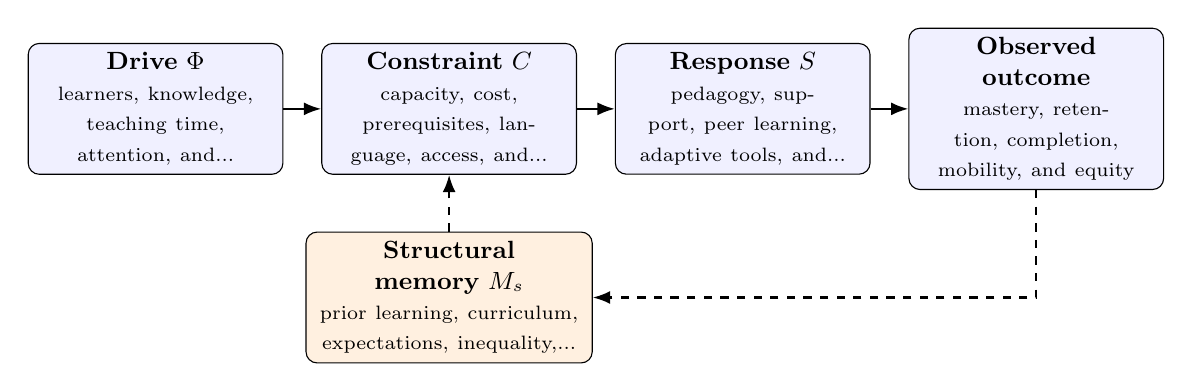
\begin{tikzpicture}[
    node distance=0.48cm,
    every node/.style={font=\small},
    box/.style={draw, rounded corners, align=center, minimum height=1.45cm, text width=3.0cm, fill=blue!6},
    memory/.style={draw, rounded corners, align=center, minimum height=1.25cm, text width=3.4cm, fill=orange!12},
    flow/.style={-{Latex[length=2.2mm]}, thick},
    feedback/.style={-{Latex[length=2.2mm]}, thick, dashed}
]
\node[box] (drive) {\textbf{Drive $\Phi$}\\\scriptsize learners, knowledge, teaching time, attention, and...};
\node[box, right=of drive] (constraint) {\textbf{Constraint $C$}\\\scriptsize capacity, cost, prerequisites, language, access, and...};
\node[box, right=of constraint] (response) {\textbf{Response $S$}\\\scriptsize pedagogy, support, peer learning, adaptive tools, and...};
\node[box, right=of response] (outcome) {\textbf{Observed outcome}\\\scriptsize mastery, retention, completion, mobility, and equity};
\node[memory, below=0.72cm of constraint] (memory) {\textbf{Structural memory $M_s$}\\\scriptsize prior learning, curriculum, expectations, inequality,...};
\draw[flow] (drive) -- (constraint);
\draw[flow] (constraint) -- (response);
\draw[flow] (response) -- (outcome);
\draw[feedback] (outcome.south) |- (memory.east);
\draw[feedback] (memory.north) -- (constraint.south);
\end{tikzpicture}
\caption{Paper C-06 observable CDFD/AFL architecture for Education. Solid arrows give the proposed forward chain; dashed arrows make history-dependent feedback explicit.}
\label{fig:c06-architecture}
\end{figure}

\subsection{Minimal Coupled Model}

A paper-level model must separate throughput, constraint accumulation, response,
and history. One deliberately minimal form is
\begin{align}
Y(t) &= \frac{\Phi(t)S(t)}{\epsilon + C(t)}, \\
\frac{dC}{dt} &= \alpha \Phi(t) - \beta S(t)C(t) + \gamma \mathcal{L}C(t), \\
\frac{dM_s}{dt} &= \eta C(t) - \mu M_s(t), \\
\Psi_s(t) &= \frac{\widehat{\Phi}(t)}{\epsilon+\widehat{C}(t)}\,
             \widehat{S}(t)\,[1+\omega\widehat{M_s}(t)] .
\end{align}
Here $Y$ is the measured output, $\epsilon>0$ prevents a singular denominator,
$\mathcal{L}$ is a spatial or network coupling operator, and hats denote
explicitly normalized variables. The sign and magnitude of $\omega$ must be
estimated: memory can preserve useful organization or amplify damage. No fixed
threshold is universal before the variables, normalization, and observation
scale are declared.

For this paper, the hypothesized causal sequence is specific. A change in
learners, knowledge, teaching time, attention, and credentials arrives faster than pedagogy, support, peer learning, adaptive tools, and institutional change can compensate.
This raises or redistributes capacity, cost, prerequisites, language, access, and assessment. If the load persists,
the retained state encoded by prior learning, curriculum, expectations, inequality, and institutional history changes the next response, so a later event of equal
magnitude can produce a different trajectory in mastery, retention, completion, mobility, and equity. The
scientific task is to estimate that sequence against the best ordinary model of
the domain, not merely to redescribe the outcome after it occurs.

\subsection{Cross-Scale Universality Without Mechanistic Erasure}

For the socioeconomic systems family, the universal comparison is between human and institutional throughput, unequal access to capacity, adaptive coordination, and historical path dependence. The variables are not morally neutral: aggregation can hide who receives flow, who bears constraint, and whose prior losses become persistent memory. \cite{BarabasiAlbert1999,WattsStrogatz1998,Holling1973,Shannon1948}
The CDFD programme is cumulative: Part I supplies the flow--constraint
foundation \cite{MujjabiPartI2026}; Part II asks when maintained throughput
supports persistent organized states \cite{MujjabiPartII2026}; Part III
develops adaptive limitation and biological memory \cite{MujjabiPartIII2026};
and Part IV \cite{MujjabiPartIV2026} tests how much of that architecture
survives translation. The CDFD Runtime \cite{CDFDRuntime2026} supplies a
reproducible numerical stress surface, but it does not substitute for the
domain evidence named here.

The required scale declaration for this paper is minutes to generations; classrooms to education systems. At short
scales, the key question is whether the incoming drive is transmitted,
buffered, or diverted. At intermediate scales, response changes effective
capacity and network exposure. At long scales, retained structure can alter the
state space itself. A result is genuinely cross-scale only when the aggregation
rule is stated and the same conclusion is not an artifact of averaging.

\subsection{Evidence Ladder and Discriminating Tests}

\begin{table}[htbp]
\centering
\small
\caption{Evidence ladder for Paper C-06. Each rung can fail independently.}
\begin{tabularx}{\textwidth}{|p{0.17\textwidth}|X|X|}
\hline
\textbf{Test} & \textbf{Design} & \textbf{Discriminating result} \\
\hline
Proxy audit & Measure longitudinal learning data, attendance, assessments, interventions, and resource records and preregister how each record maps to $\Phi$, $C$, $S$, $M_s$, and $Y$. & The mapping fails if proxies are non-identifiable, circular, or change meaning across cases. \\
\hline
Load ramp & Apply or observe a curriculum, staffing, or access change across different prior-learning states while estimating the dominant constraint and response time. & A threshold claim requires a reproducible nonlinear change and uncertainty bounds, not a visually chosen breakpoint. \\
\hline
Recovery and memory & Match present load across units with different histories, then compare recovery paths. & The memory claim requires history-dependent divergence after current conditions are controlled. \\
\hline
Model comparison & Compare the baseline domain model with and without the CDFD/AFL state variables using held-out data. & The paper's stated falsifier is: history-sensitive CDFD variables do not improve learning or completion prediction. \\
\hline
\end{tabularx}
\end{table}

The strongest practical design combines a prospective perturbation with a
recovery window. The load-ramp phase estimates where constraint begins to rise
faster than output. The recovery phase estimates $\beta$ and $\mu$, separating
fast relaxation from persistent memory. A topology or coupling intervention
then asks whether rerouting changes the cascade as predicted. Null results are
informative because they identify domains in which the universal notation adds
no measurable value.

\subsection{Research Programme and Boundary Conditions}

The immediate research programme has four steps. First, construct a documented
dataset from longitudinal learning data, attendance, assessments, interventions, and resource records and retain raw units before normalization.
Second, fit a baseline domain model and report its calibration and out-of-sample
error. Third, add the smallest identifiable CDFD/AFL state extension and test
whether it improves prediction of mastery, retention, completion, mobility, and equity. Fourth, repeat the
analysis across the declared scale range and publish negative cases as part of
the universality audit.

Three boundaries are non-negotiable. Correlation between flow and failure does
not identify a constraint mechanism. A fitted memory term does not prove that
the stored state has the same material meaning in another domain. Finally, a
runtime cascade is evidence about the implementation, not evidence that the
real system follows it. The paper becomes stronger when it can say precisely
where the translation stops.


% END PART IV MAJOR UNIVERSAL UPGRADE

\section{Conclusion}
Education can be studied as constrained knowledge transfer with strong institutional memory. The CDFD hypothesis is that some forms of over-constraint reduce learning and adaptation; the test is whether the declared variables improve prediction without treating reform or disruption as inevitable.
\section*{Conflict of Interest} The author declares no conflict of interest.
\section*{Data Availability}
Part-specific runtime diagnostics are under each Part's \path{outputs/} directory.

Release-wide code: \path{Part_E_Synthesis/supplementary/}.

Generated summaries: \path{Part_E_Synthesis/outputs/}.

Figures: \path{Part_E_Synthesis/figures/}.


\section{Reference Layer}
\bibliographystyle{plain}
\bibliography{universal_afl_references}
\end{document}
